\chapter[Simulation]{Simulation}
\label{chapter:Result}

%\section{System Model}

%\section{Simulation Results}

\section{Received Power detection}
In this section, the proposed received power detection using the CUSUM and GLR algorithm discussed above is introduced. 

First, the statistics $g_t$ calculation results related to the sample ID using the probability density ratio $l_0(y)$ and $l_1(y)$ are shown in Figs.\ref{OFF2ON} and \ref{ON2OFF}, respectively. The rise up point is set to be the 512th sample and the rise down point is set to be 1532th sample.
In Figure \ref{OFF2ON}, when a status of the primary user from OFF to ON changes, the statistic $g_t$ shows a increase trend, and when the status changes from ON to OFF, a decrease trend is shown. The reason is that if the probability density ratio $l_0(y)$ is used to calculate the statistics $g_t$, the ON samples show a positive trend and OFF samples a negative trend. Then in this case, the statistics $g_t$ exceeds the threshold $h$, the rise up point is declared to be detected.

Samely, in Figure \ref{ON2OFF}, when a status of the primary user from OFF to ON changes, the statistic $g_t$ shows a increase trend, and when the status changes from ON to OFF, a decrease trend is shown. The reason is that if the probability density ratio $l_1(y)$ is used to calculate the statistics $g_t$, the ON samples show a negative trend and OFF samples a positive trend. Thus, the statistics $g_t$ exceeds the threshold $h$, the rise down point is declared to be detected.

Based on the detected rise up and rise down point, an active period of the primary user is extracted to calculate the received power. Since the only ON samples is detected to be used for calculating the received power, it may mitigate the sensing error compared with not considering ON sample extraction.

\begin{table}[t]
\begin{center}
 \caption{\normalsize{Simulation parameters}}
 
\normalsize

  \begin{tabular}{c|c}
    & \\
    Parameter &Value \\ \hline
    SNR & -10〜20[dB] \\
    $[P_{{\rm min}},P_{{\rm max}}]$ & [$P$/2, 2$P$] \\
    $\sigma^2$ & 1 \\
    sample number & 2048 \\
    $\bar{T}_0$ & 10 \\
    transition partern & OFF $\rightarrow$ ON $\rightarrow$ OFF \\
    rise up point & 512th sample\\
    rise down point & 1536th sample\\
    Number of trials & 10,000 \\ \hline
  \end{tabular}
\label{parameter}
\end{center}
\end{table}
\section{Simulation results and performance evulation}
In this section, we use computer simulation to evaluate the performance of transition point detection and the received power detection using CUSUM and GLR algorithm. The simulation parameters are shown in Table \ref{parameter}.

To vertify the performance of the received power, we evalate

\begin{enumerate}
\item the performance of the rise up point and the rise down point detection, 
\item the performance of the received power detection using the detected transition point.
\end{enumerate}
Figures \ref{transition_up} and \ref{transition_down} show the boxplot results of detected rise up point and rise down point respectively. The body of the boxplot consists of a box, which goes from the fisrt quartile to the third quartile. The line drawn at the box means the median of the detected transition point. The lines extended from the box called whiskers mean the smallest and the largest nonoutlier from the box. The real rise up point and rise down piont are fix on the 512th sample and 1532th sample. From the simulation results, we can see that in low SNR region the variation of transition point is large, howerver, in high SNR region the detected transition point converges to the real one.

\newpage

\begin{figure}[t]
\centering
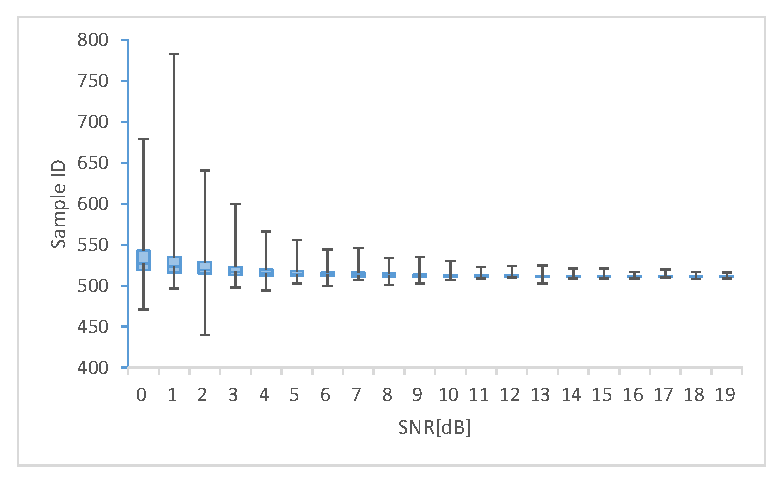
\includegraphics[width=100mm]{transition_up.eps}
\caption{Boxplot result of the rise up point.}
\label{transition_up}
\end{figure}
\begin{figure}[t]
\centering
\includegraphics[width=100mm]{transition_down.eps}
\caption{Boxplot result of the rise down point.}
\label{transition_down}
\end{figure}

Figures \ref{Powdiff} shows the performance of the power difference with the real power. 
The received power detection without considering ON/OFF transition during the sensing period, which means the all samples is used for calculating the received power, is considered as a conventional method for comparison. The dotted line means that the ideal case that the real received power is detected exactly. The power difference $P_{\rm diff}$ with real power is defined as follows,
\begin{eqnarray}
P_{{\rm diff}} &= P-P_{{\rm ON}}.
\label{diff}
\end{eqnarray}

The simulation result shows that the proposed method for the received power detection using CUSUM algorithm and GLR algorithm can obtain a better performance than the conventional method. In low SNR region, the proposed method can achieve 0.5[dB] gain than the conventional one, and in high SNR region, 1.3[dB] is improved.

\begin{figure}[t]
\centering
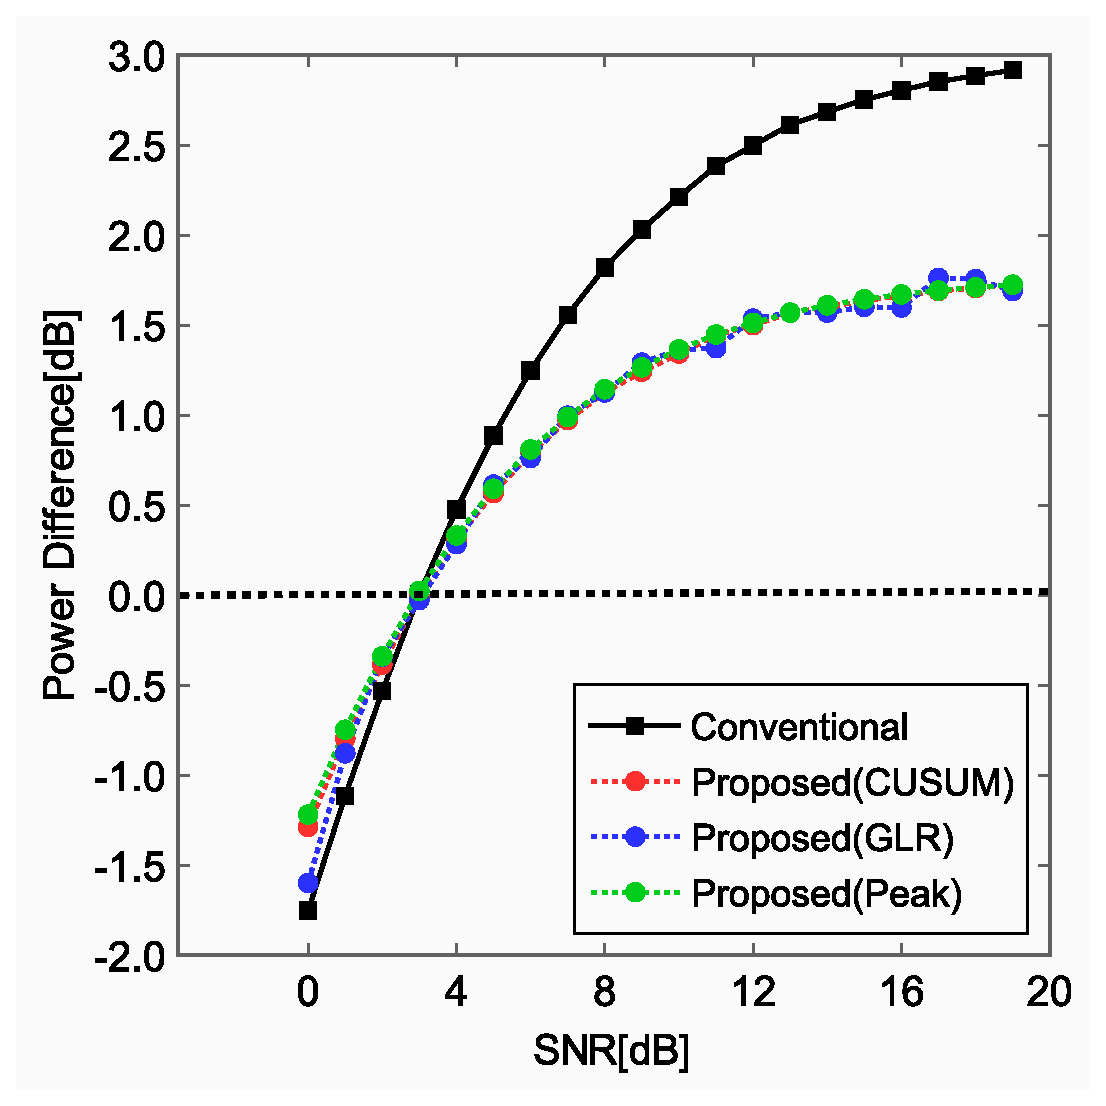
\includegraphics[width=100mm]{peak.eps}
\caption{The power difference with the real power.}
\label{Powdiff}
\end{figure}

\begin{figure}[t]
\centering
\includegraphics[width=100mm]{cdf_OFF2ON.eps}
\caption{CDF of rise up point detection(rise up point is set to be 500th sample).}
\label{cdf_off2on}
\end{figure}


\begin{figure}[t]
\centering
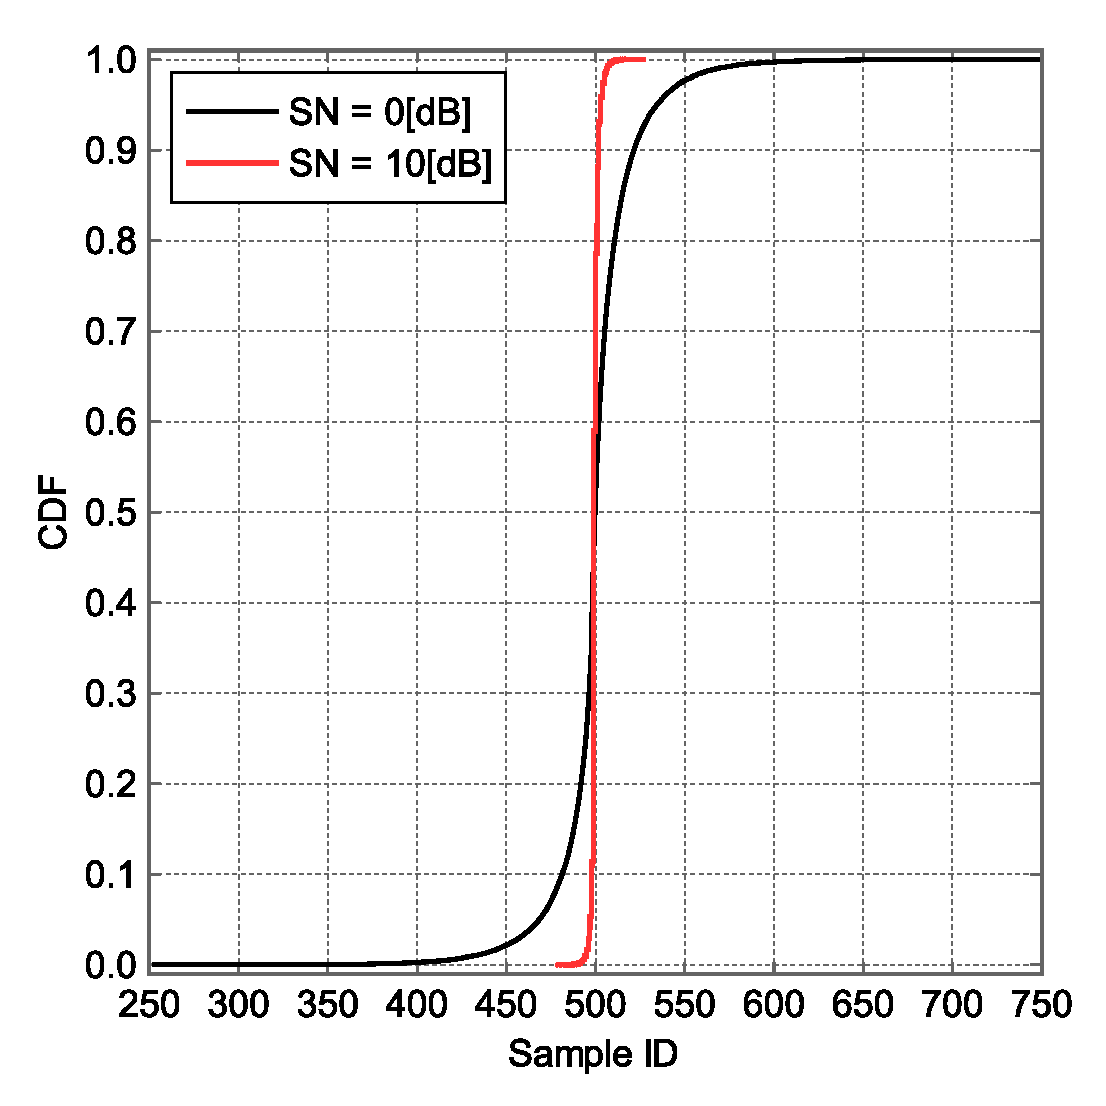
\includegraphics[width=100mm]{cdf_ON2OFF.eps}
\caption{CDF of rise down point detection(risen down point is set to be 1500th sample).}
\label{cdf_on2off}
\end{figure}


\begin{figure}[t]
\centering
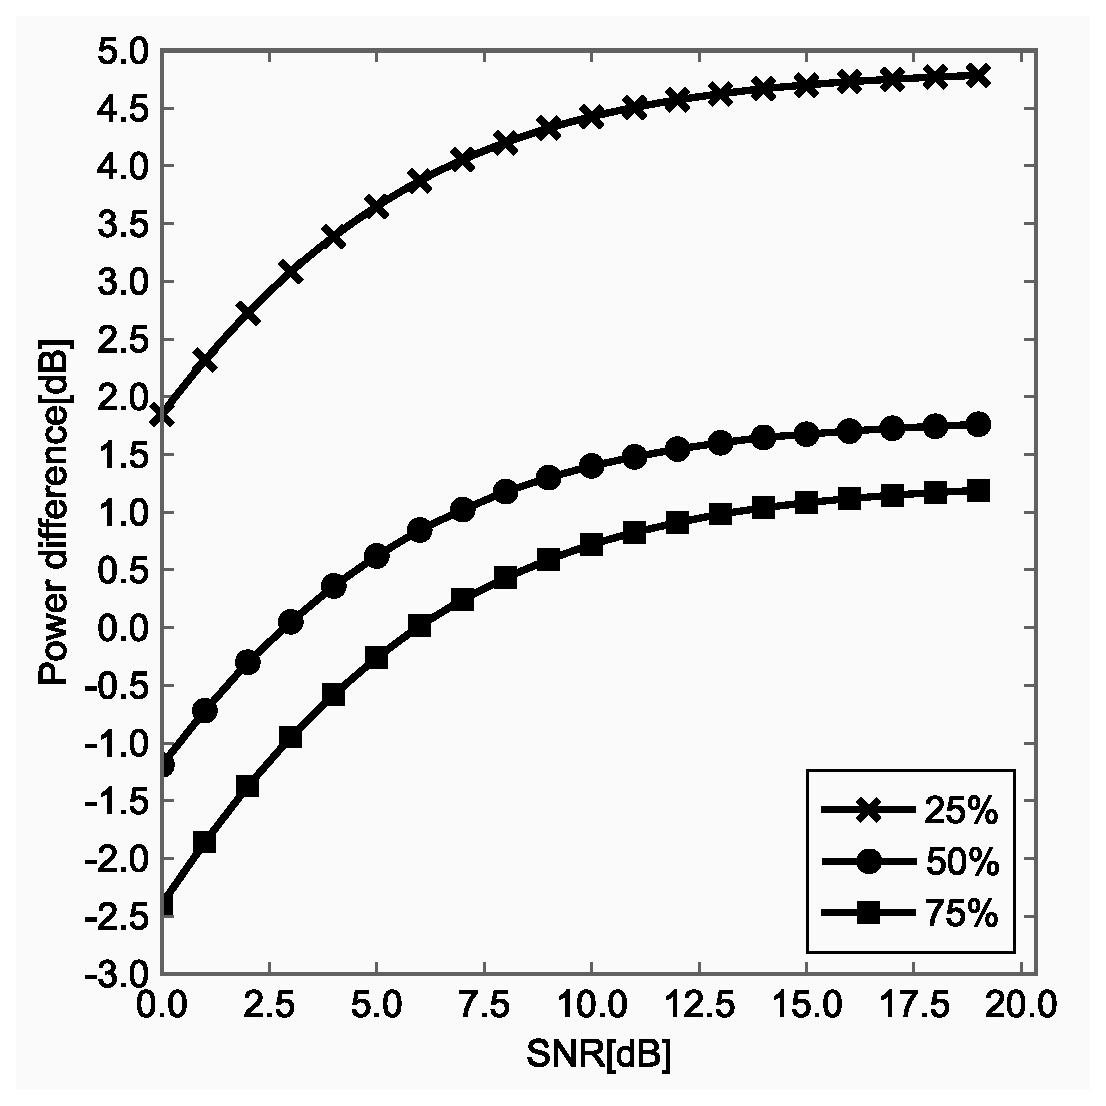
\includegraphics[width=100mm]{per.eps}
\caption{The power difference with the real power at different ON percentage during the sensing period.}
\label{per}
\end{figure}
